%%%%%%%%%%%%%%%%%%%%%%%%%%%%%%%%%%%%%%%%%%%%%%%%%%%%%%%%%%%%%%%%%%%%%%%%%%%%%%%%%%%%%%%%%%
\section{Methods}
\paragraph{Resources Hyperlinks} 
\begin{itemize}
    \item \href{https://www.kaggle.com/code/rafjaa/dealing-with-very-small-datasets}{Dealing with very small datasets | Gaggle}
    
\end{itemize}


%%%%%%%%%%%%%%%%%%%%%%%%%%%%%%%%%%%%%%%%%%%%%
\subsection{Dataset}


Our dataset and all the source code can be found in the following gihtub
repository. 

Our dataset contains 14 features extracted on XXX:n different lymphoma. Each
feature is extract from a PET Scanner XXX: type where different image
reconstruction techniques was applied. In our analysis we will study 3
different reconstruction methods, XXX: names. This will be our classification
targets. Thus, we are interested to see if it is possibly to identify features
that gives good class separation with respect to reconstruction method. This
will be a challenging since our data only contains 16 samples per
reconstruction. This will be an exercise in selecting good features applied to
simple ML models


%%%%%%%%%%%%%%%%%%%%%%%%%%%%%%%%%%%%%%%%%%%%%
\subsection{Random forest}
In our first attempt to identify good features (features with good
class separation), we will use a random forest classifier. 
It can be used to identify the features and feature value that splits the data
into the purest classes (see XXX)
The algorithm works by constructing multiple decision trees, each of which is trained 
on a subset of the data. 

\subsubsection{Decision Tree Classifier}
A classification decision tree is a predictive model that predicts the target
class of a feature based on a set of binary rules . The decision tree consists of a series of
nodes, branches, and leaves. Each node represents a decision point, each branch
represents a possible outcome, and each leaf represents a final consequence or
result. 

% XXX: explain fig
% and structure in a decision tree
\begin{figure}[H]
    \centering
    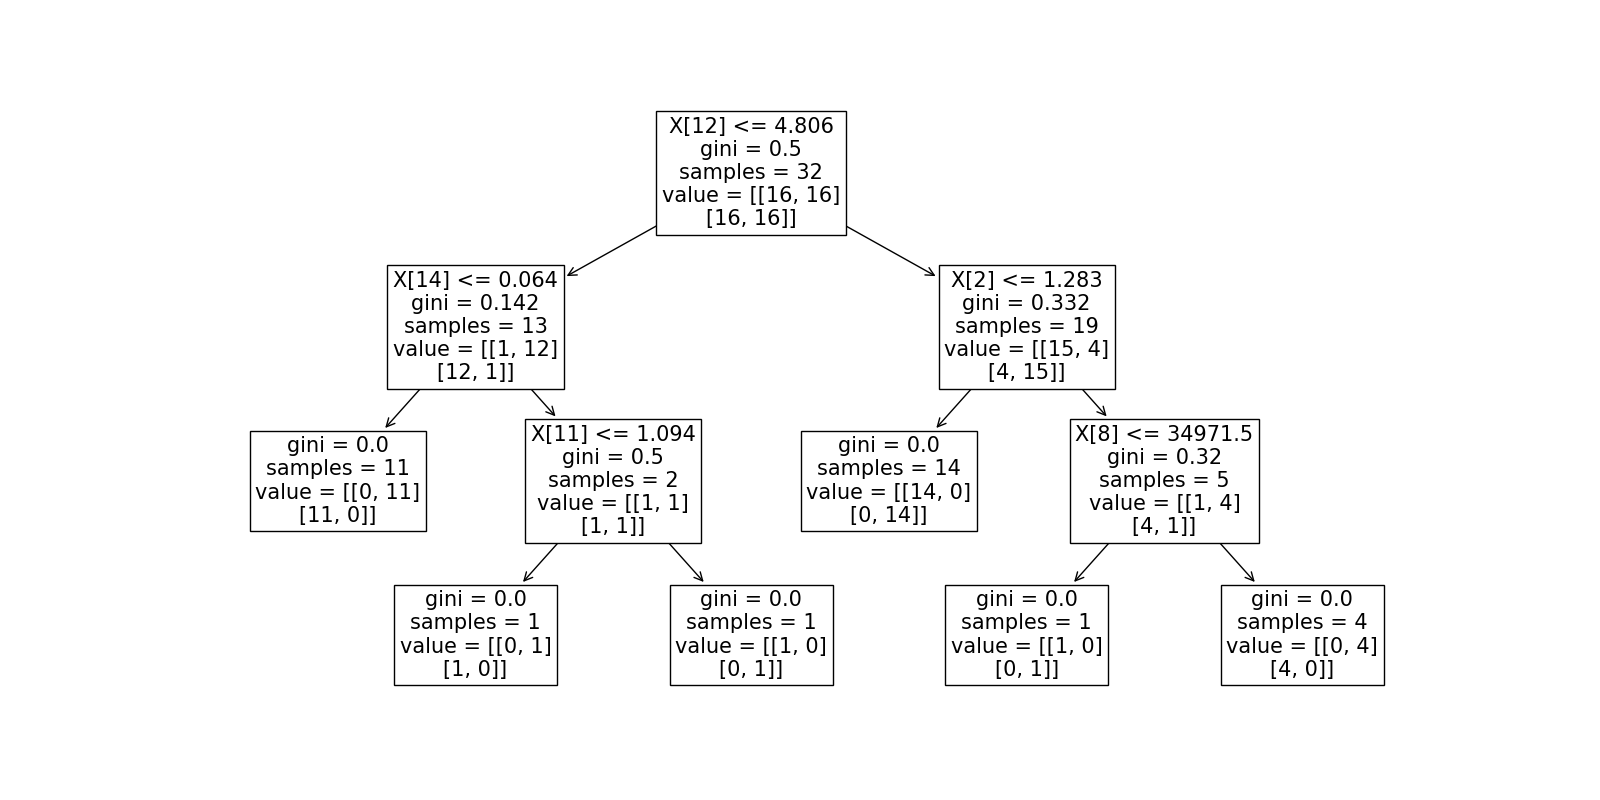
\includegraphics[width=0.8\textwidth]{Figures/descion_tree.png}
    \caption{Decision tree}  
    \label{fig:descision_tree} 
\end{figure}

A typical structure of a decision is shown in figure \ref{fig:descision_tree}. Each rectangle
represents a node in the tree. The build of a decision consists of finding
the feature and feature value (threshold) at each node that maximizes the
purity of each child node resulting from the split. At each node the data is
split into two child nodes based on the threshold value. Values lower than the threshold is
passed to the left child node and values higher is passed to the right child
node. Thus, the tree consists of a set of rules on where to a specific sample. The algorithm is recursive and starts at the
root node (the upper rectangle) on continues until a Leaf node is reached.
That is, one of the squares in the bottom of the figures.     


\paragraph{The CART algorithm} \hfill

We implemented the CART algorithm to find the optimal splits in the data.  

The CART algorithm splits the data set in two subsets using a single feature
$k$ and a threshold $t_k$ \cite{w44}. The purity of the split is then evaluated
with the cost function: 
\begin{equation*}
    \label{eq:cart} 
    C(k, t_k) = \frac{m_{\text{left}} }{m} G_{\text{left}}+
    \frac{m_{\text{right}} }{m} G_{\text{right}}, 
\end{equation*}

where $G$ is a measure of impurity (see section ),
$m_{\text{left}} $ and $m_{\text{right}} $ is the number of samples in the left
and right subsets resulting from the split. The total number of samples is $m =
m_{left} + m_{right}  $ 

The algorithm iterates through all p features and n samples. For each feature k
and threshod $t_k$, the cost score is evaluated on the two subsets. The
threshold and features that produced the best score is stored in a node. This
process is repeated on the data subsets in a recursive way until a specific
criterion is met. This produces a leaf node in the tree. 

In our implementation the recursion stops if it is not possible to split the
subset further. That is, the number of samples in the subset is equal to one.   
The recursion will also stop if our subset is 100\% pure. That is, the subset
only consist of one class label.  

\paragraph{Gini factor} \label{sec:gini_factor} \hfill

The Gini factor is used to measure the purity of the data subset and is
calculated as:
\begin{equation*}
    G = 1 - \sum_{i=1}^{c} P_i ^2 
\end{equation*}
where $P_i$ is the probability that a sample belongs to class i. 

For a maximum impurity, where $P_1 = P_2 = 0.5$ the Gini factor is 0.5. A
smaller value indicates a better split. For a perfectly pure class the Gini
factor is 1. That is all the samples belongs to a class k ($P_k = 1$).     


Our class target labels was stored in one hot vector of size $n \times c$, 
where n is the number of samples in the data subset and c is the number of
classes. The probability of each class was calculated with this python snippet:
\begin{lstlisting}[language=Python]
import numpy as np
P = np.sum(y, axis = 0)/y.shape[0]
\end{lstlisting},
where \verb|y| is the one hot vector of our class targets. 

\paragraph{Calculating the feature importance} \hfill
Our random forest implementation was used to identify most discriminative
features and not used for its predictive power. Again, we will use the Gini
factor to calculate the feature importance. 


We want to quantify the impurity decrease as results of a feature split.
Therefore, we are interested in the change in impurity with respect to a node and its
child nodes. The impurity decrease also needs to take into account the number
of samples. A feature is more important if it is able to separate more samples.       

% We will use the same formula as the scikit learn python library \cite{sklearn}
to estimate the feature importance: 
\begin{equation*}
    \frac{m}{M} \cdot (G  - \frac{m_{\text{left}} }{m} G_{\text{left}}+
    \frac{m_{\text{right}} }{m} G_{\text{right}}), 
\end{equation*}
where $G$, $G_{left} $ and $G_{right} $ as the Gini factor for the parent,
left child and right child node respectively. M is the total number of samples
in our input data. The other quantities are as defined in equation
\ref{eq:cart}. 

All our decision trees has a variable called \verb|feature_importances_|, which
contains the impurity decrease obtained from the best split of a node (except
for leaf nodes).   

When building the tree all features is considered each time a node is to be
split. If the same feature is used multiple times to split nodes in to a tree.
Then, only the split that produces the highest impurity decrease is stored in
the \verb|feature_importances_| variable. Hence, used to evaluate the feature
importance.      



Our decision tree algorithm can be used directly to identify good features.
However, there are some problems. The algorithm usually produces very different
results dependent on small variations in the data. That is, classification
decision trees suffers from high variance. It may also neglect highly
correlated features that produces a slightly poorer separation. To circumvent
these problems we implemented the random forest algorithm. 

%%%%%%%%%%%%%%%%%%%%%%%%%%%%%%%%%%%%%%%%%%%%%
\subsection{Random forest}
Random forest is a type of ensemble learning method, which uses multiple
decision trees to make predictions and combines them to create a more accurate
and stable prediction. It uses a technique called bagging, which involves
randomly selecting a subset of data from the training set and building a
decision tree from each subset. 

It also uses feature resampling to reduce the
overfitting of the model. We will implement feature resampling
to better evaluate the performance of all the features. Feature resampling is
done within each node of the descion tree. Hence, the best split at each node is
evaluated on different feature subsets. The general algorithm for a descion
tree is listed below. 
\paragraph{Algorithm} 

% Random forest algorithm - cite lecture 44
\fbox{\begin{minipage}{30em}
We will grow of forest of say $\bm{B}$ trees.

For b=1:B

Draw a bootstrap sample from the training data organized in our $\boldsymbol{X}$ matrix.

We grow then a random forest tree $T_b $
based on the bootstrapped data by repeating the steps outlined till we reach
the maximum node size is reached

we select $m \leq p$  variables at random from the p predictors/features

pick the best split point among the $m$ features using for the CART
algorithm and create a new node

split the node into daughter nodes

Output then the ensemble of trees $\{T_b\}^B_1$

and make predictions for either a regression type of problem or a
classification type of problem.


\end{minipage}}

















% What is one hot vector?
% A one hot vector is a vector of all zeros, except for a single element which is set to one. 
% It is commonly used to represent a categorical variable in machine learning models.


1. Start by selecting the best attribute from the dataset. This attribute will be the root node of the decision 
tree. 

2. Split the data into subsets based on the attribute selected in the first step. 

3. For each subset, select the best attribute and create a decision tree node.

4. Repeat the process for each subset until all the data points have been classified.

5. Finally, test the accuracy of the decision tree by running it on a different set of data.
















\paragraph{Overview} 
\begin{enumerate}
    \item Identify good features by visual inspection 
    \item Feature reduction:
        \begin{itemize}
            \item Manual:
                \begin{itemize}
                    \item Remove correlated features
                \end{itemize}
                
            \item Automatic:
                \begin{itemize}
                    \item Iterate all the features and find best model 
                \end{itemize}
                
        \end{itemize}
        
    \item Evaluate results and find the best ML classification algorithm for dataset 
    
\end{enumerate}


%%%%%%%%%%%%%%%%%%%%%%%%%%%%%%%%%%%%%%%%%%%%%
\subsection{Feature section}
\begin{itemize}
    \item not correlated
    \item highly dependent on target variable 
\end{itemize}




%%%%%%%%%%%%%%%%%%%%%%%%%%%%%%%%%%%%%%%%%%%%%
\subsection{Dataset and model selection}
\begin{itemize}
    \item Bagging - Bootstrap aggregation
    \item Random forest
\end{itemize}

\begin{itemize}
    \item Sparse data $ \rightarrow $ Focus on simple ML methods
    \item ML classification algorithms suited for sparse data: 
        \begin{itemize}
            \item SVM
        \end{itemize}
        
\end{itemize}



\paragraph{ANOVA} 
Used to select features that is highly dependent on the target variable
\cite{anova}. 











\subsubsection{SVM}








